%% example.tex
%% Copyright 2010 Mohamed El Morabity
%
% This work may be distributed and/or modified under the conditions of the LaTeX
% Project Public License, either version 1.3 of this license or (at your option)
% any later version. The latest version of this license is in
% http://www.latex-project.org/lppl.txt and version 1.3 or later is part of all
% distributions of LaTeX version 2005/12/01 or later.
%
% This work has the LPPL maintenance status `maintained'.
% 
% The Current Maintainer of this work is Mohamed El Morabity
%
% This work consists of all files listed in manifest.txt.

\documentclass[11pt,xcolor=table]{beamer}

\usepackage[italian]{babel}
\usepackage{listings}
\usepackage{microtype}
\usepackage{textcomp}
\usepackage[T1]{fontenc}
\usepackage[utf8]{inputenc}
\usepackage{tikz}
\usepackage[abs]{overpic}
\setlength\unitlength{1mm}
\graphicspath{{OMV},{OC}}
\graphicspath{{percorso1},{percorso2}} 

\usetheme[language=italian]{Laughlin}

\newcommand{\acronym}[1]{\textsc{\lowercase{#1}}}
\newcommand{\command}{\texttt}
\newcommand{\email}[1]{\href{mailto:#1}{\texttt{#1}}}
\newcommand{\familyname}{\textsc}
\newcommand{\filepath}{\texttt}
\newcommand{\latexcode}{\texttt}
\newcommand{\parameter}[1]{\textlangle #1\textrangle}

\lstset{basicstyle=\ttfamily,keywordstyle=\color{laughlinblue}\bfseries,commentstyle=\color{laughlinblue!75}\itshape,columns=flexible}

\rowcolors{1}{laughlinblue!50}{laughlinblue!30}

\hypersetup{urlcolor=laughlinblue}

\title[Nas... e molto di più!]{Dispositivi per l'archiviazione in rete (NAS)... \\ e molto di più!}
\subtitle{Soluzioni Open Source Home \& Small Business}
\author{\textsc{Giuseppe Chellini}}

\institute[GULP]{GULP - Gruppo Utenti Linux Pisa}

\date{17 Febbraio 2016}

\begin{document}

	\begin{frame}
		\titlepage
	\end{frame}

\section{Introduzione}

\subsection{Il passato remoto...}

\begin{frame}
	\frametitle{Il passato remoto...}
	Negli ultimi 20 anni sono radicalmente cambiate le esigenze legate alla conservazione e gestione dei dati in formato elettronico.\\
	\vspace{0.3cm}
	Prima:
	\begin{itemize}
		\item era necessario salvare essenzialmente documenti, programmi (di piccole dimensioni), immagini;
		\item erano sufficienti pochi Floppy Disk (poi CD... poi DVD...) per archiviarli;
		\item per avere una maggiore sicurezza, si salvavano semplicemente più copie...
	\end{itemize}
\end{frame}

\subsection{... il passato recente ...}

\begin{frame}
	\frametitle{... il passato recente...}
	
	L'utilizzo di documenti multimediali è entrato a far parte della vita quotidiana \textit{(libri, riviste, musica, films)}.\\ 
	Di conseguenza, è aumentata la quantità di memoria necessaria per archiviare le informazioni.\\
	
	\vspace{0.3cm}
	... poi:
	\begin{itemize}
		\item si è diffuso l'uso di HD esterni per la conservazione di documenti e materiale multimediale;
		\item in questo periodo si utilizzavano PC fissi o portatili per la fruizione dei contenuti;
		\item prime unità dedicate per l'ascolto di musica (\textit{iPod,...}) e visione di film (\textit{PSP...}) attraverso le loro versioni digitali su supporto DVD o USB.
	\end{itemize}
\end{frame}

\subsection{... ed il presente!}
\begin{frame}
	\frametitle{... ed il presente!}
	
	Con la diffusione di dispositivi capaci di utilizzare materiale disponibile attraverso la rete (\textit{Consolle, lettori multimediali, smartphone,...}) è sorta la necessità non solo di conservare ma anche di avere e rendere disponibili i contenuti, magari a più utilizzatori contemporaneamente.\\
		
	\vspace{0.3cm}	
	... ed oggi:
	\begin{itemize}
		\item Si utilizzano smartphone e tablet (ridotta capacità di memoria) per documenti e contenuti multimediali disponibili in rete (youTube\textregistered, SoundCloud\textregistered...);
		\item Si sono diffuse piattaforme di conservazione dati in rete che permettono la condivisione dello spazio tra più utenti e su più dispositivi contemporaneamente.
	\end{itemize}
\end{frame}

\subsection{"Anatomia" di una rete locale}

\begin{frame}
	\frametitle["Anatomia" di una rete]{"Anatomia" di una rete "moderna"}
		Tipica configurazione di una abitazione (magari di studenti) o di un ufficio:
	
	\begin{center}
		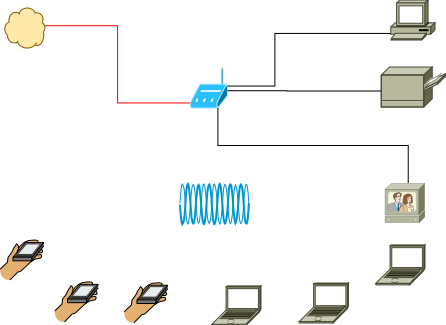
\includegraphics[width=0.8\textwidth]{SchemiRete/AnatomiaReteNoNas.png}
	\end{center}
\end{frame}

\begin{frame}
	\frametitle["Anatomia" di una rete]{"Anatomia" di una rete "moderna"}
	Configurazione arricchita da un "NAS"
	\begin{center}
		\begin{overpic}[width=0.8\textwidth]{SchemiRete/AnatomiaRete.png}
			\put(5,21){NAS}
		\end{overpic}
	\end{center}
\end{frame}
	
\begin{frame}
	\frametitle[Definizione di "NAS]{Definizione di "NAS"}
	\begin{block}{da Wikipedia:}
		Un \textit{Network Attached Storage} (NAS) è un dispositivo collegato alla rete la cui funzione è quella di consentire agli utenti di accedere e condividere una memoria di massa, in pratica costituita da uno o più dischi rigidi, all'interno della propria rete o dall'esterno.
	\end{block}
	\vspace{3mm}
	Un NAS è dunque composto da:
	\begin{description}
		\item[Hardware] macchina dotata dello spazio fisico per la memorizzazione (uno o più dischi) ed il collegamento alla rete;
		\item[Software] sistema operativo per la gestione della memorizzazione e dei servizi.
	\end{description}
\end{frame}

\begin{frame}
	\frametitle{Alcune caratteristiche dei "NAS"}
	
	\begin{block}{Gestione dei dischi}
	\textbf{RAID} "Redundant Array of Indipendent Disks" \footnote{Sistema ridondante di dischi indipendenti}\\
	Sistema di “connessione logica” tra più dischi per ottenere determinati vantaggi, quali:
		\begin{itemize}
			\item la visione unica di tutto lo spazio disponibile
			\item l’aumento delle prestazioni in lettura/scrittura
			\item l’aumento della sicurezza dei propri dati
		\end{itemize}
	\end{block}
	
	\begin{block}{Servizi disponibili}
		\textbf{SMB/CIFS}, NFS, FTP, TFTP, rsync, Unison, SCP (SSH), UPnP server (\textbf{MiniDLNA}), \textbf{iTunes/DAAP} server, Lighttpd (Webserver), Transmission \textbf{BitTorrent} client...
	\end{block}
\end{frame}

\section{Soluzioni commerciali}
\begin{frame}
	\frametitle{Alcune soluzioni in commercio}
	\begin{columns}
		\begin{column}{0.48\textwidth}
			\centering
			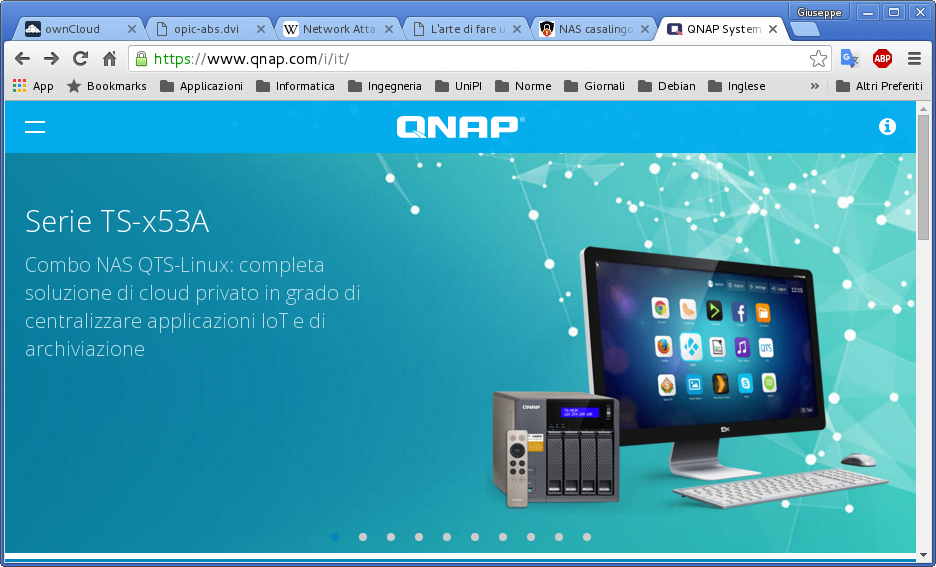
\includegraphics[width=0.8\textwidth]{NasComm/NAS1.png}
			\vspace{1mm}
			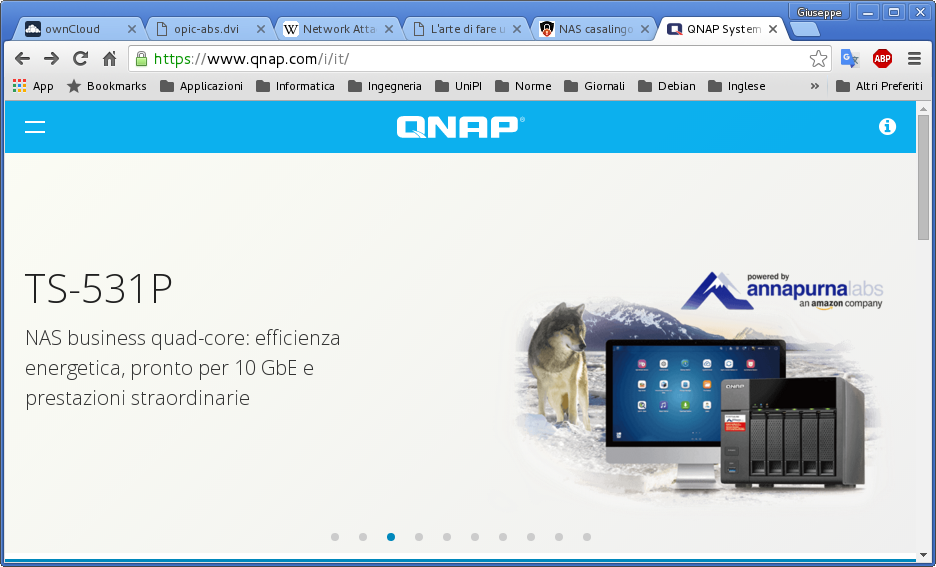
\includegraphics[width=0.8\textwidth]{NasComm/NAS2.png}
			\vspace{1mm}
			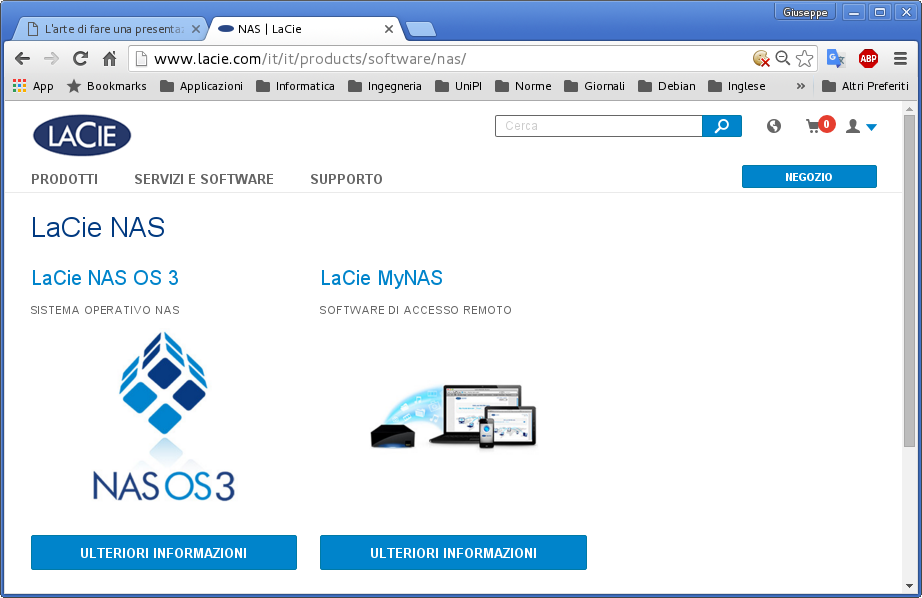
\includegraphics[width=0.8\textwidth]{NasComm/NAS5.png}
		\end{column}
		\begin{column}{0.48\textwidth}
			\centering
			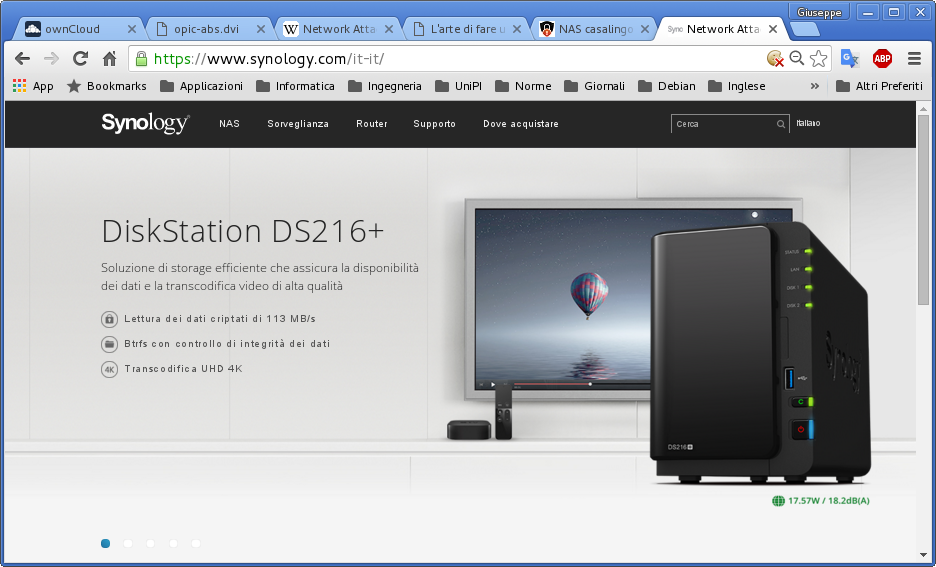
\includegraphics[width=0.8\textwidth]{NasComm/NAS3.png}
			\vspace{1mm}
			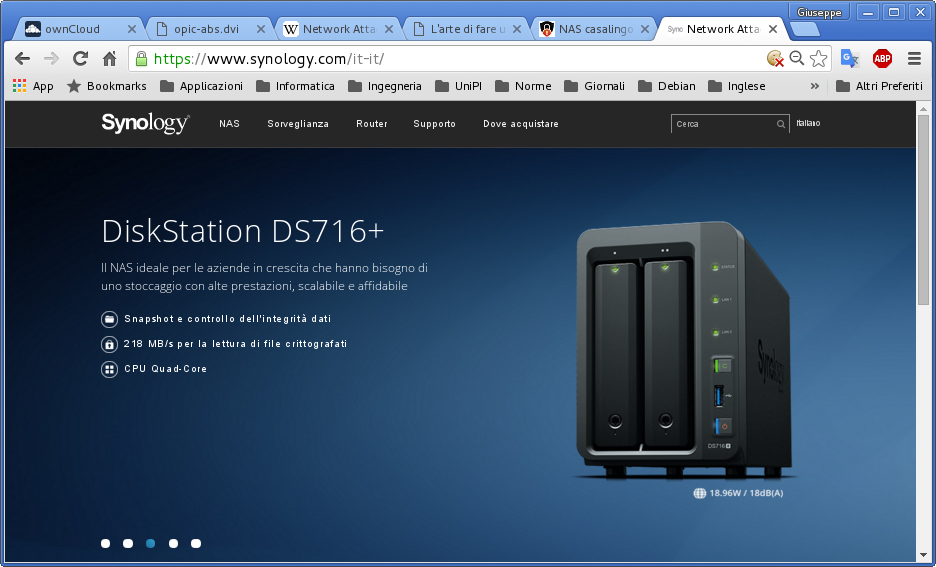
\includegraphics[width=0.8\textwidth]{NasComm/NAS4.png}
			\vspace{1mm}
			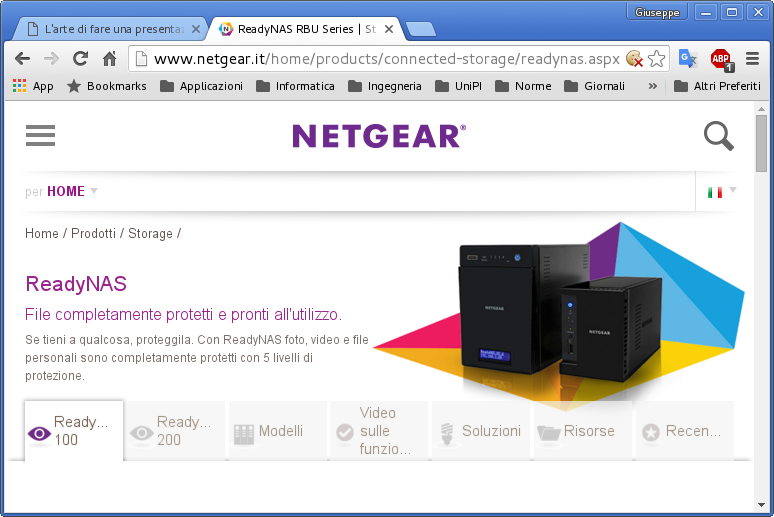
\includegraphics[width=0.8\textwidth]{NasComm/NAS6.png}
		\end{column}
	\end{columns}
\end{frame}

\section{Soluzioni Open Source}

\begin{frame}
	\frametitle{Soluzioni Open Source}
	Posso decidere di dotarmi di un NAS realizzato mediante software Open Source. In questo caso devo tenere presenti:
	
	\begin{alertblock}{Contro (se siamo qui, non ci spaventano...)}
		\begin{itemize}
			\item dovrò occuparmi prima dell'\textbf{hardware} (macchina, dischi) 
			\item dovrò gestire le fasi di \textbf{configurazione}
		\end{itemize}
	\end{alertblock}
	
	\begin{exampleblock}{Pro (se siamo qui, ci piacciono molto...)}
		\begin{itemize}
			\item potrò \textbf{riutilizzare hardware} magari non "recenti"
			\item potrò contenere la \textbf{spesa} necessaria
			\item forse potrò gestire una quantità maggiore di \textbf{opzioni senza limitazioni}
			\item potrò contare su una \textbf{comunità} che sviluppa le potenzialità del software (interfaccia e servizi)
		\end{itemize}
	\end{exampleblock}
\end{frame}

\subsection{Nas4free / FreeNAS}

\begin{frame}
	\frametitle{Soluzioni OS: Nas4free/FreeNAS}
	\begin{itemize}
		\item Sistema operativo base: \textbf{FreeBSD}
		\item Sistema grafico minimale con accesso mediante WebGUI
		\item Installabile su HD interno o su supporto USB rimovibile
		\item File system ZFS e gestione software dischi in RAID
	\end{itemize}
	\centering
	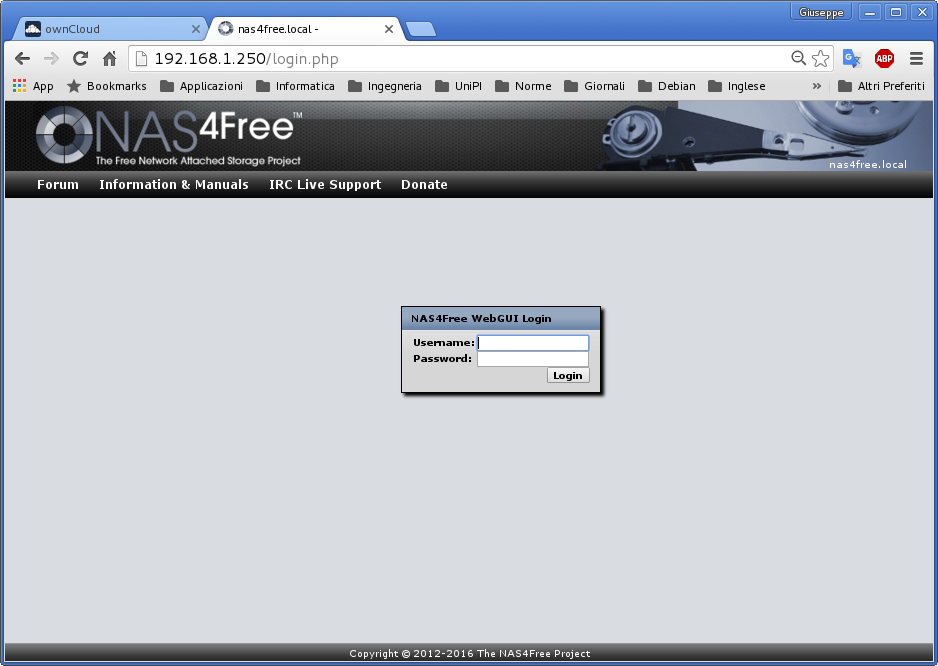
\includegraphics[width=0.7\textwidth]{N4F/N4Fscreen.png}	
\end{frame}

\begin{frame}
	\frametitle{Soluzioni OS: Nas4free (FreeNAS)}
	\begin{columns}
		\begin{column}{0.48\textwidth}
			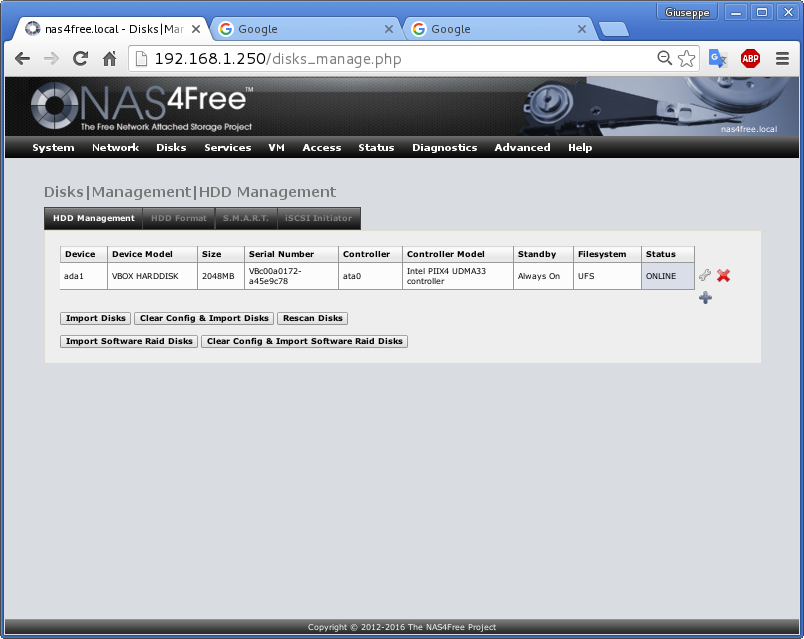
\includegraphics[width=\textwidth]{N4F/N4Fscr1.png}\\
			\vspace{3mm}
			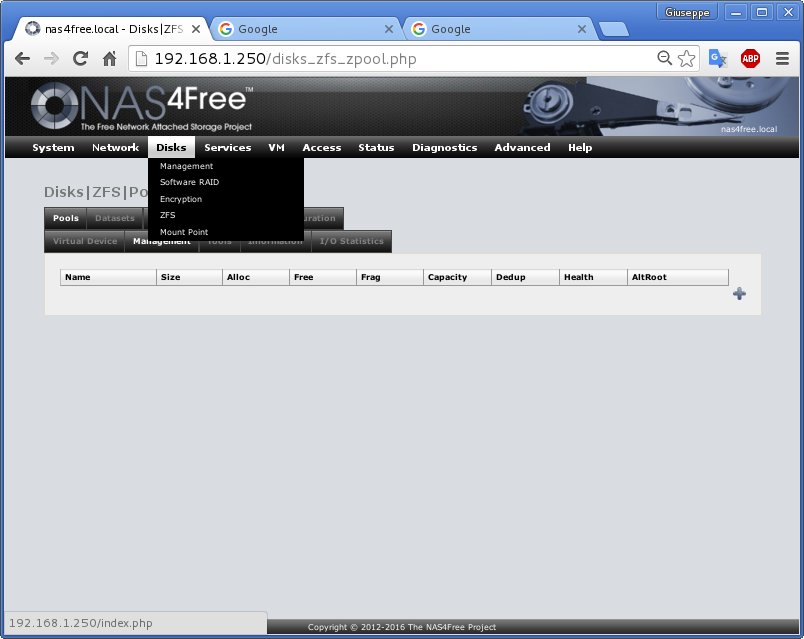
\includegraphics[width=\textwidth]{N4F/N4Fscr2.png}\\
		\end{column}
		\begin{column}{0.48\textwidth}
			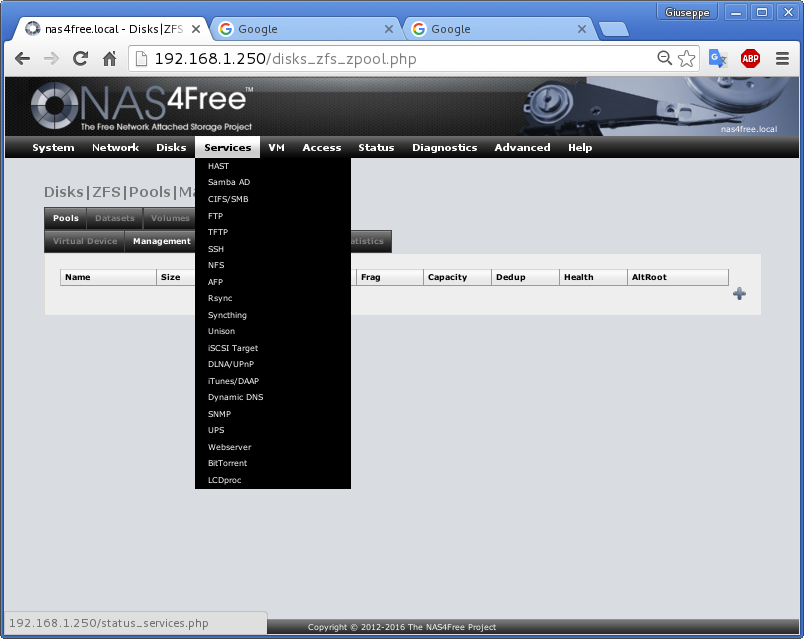
\includegraphics[width=\textwidth]{N4F/N4Fscr3.png}\\
			\vspace{3mm}
			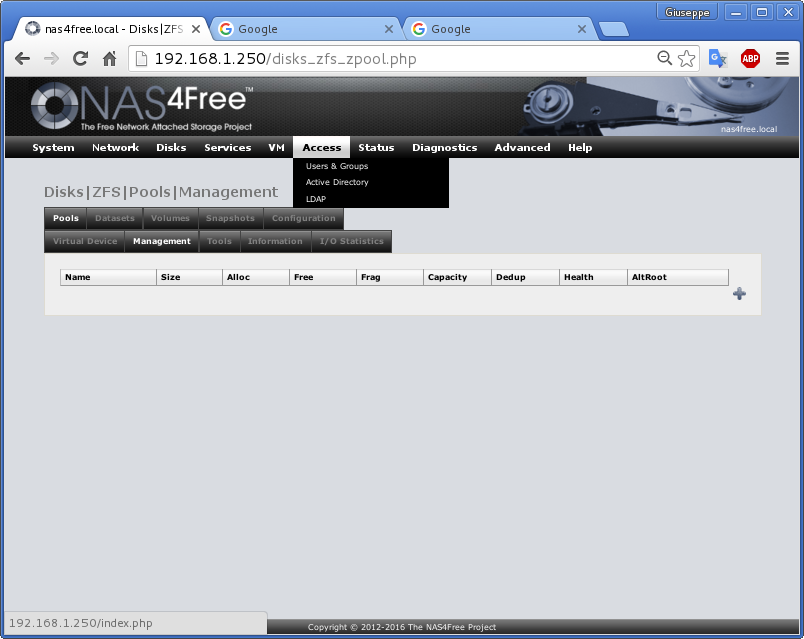
\includegraphics[width=\textwidth]{N4F/N4Fscr4.png}\\
		\end{column}
	\end{columns}
\end{frame}

\subsection{OpenMediaVault}

\begin{frame}
	\frametitle{Soluzioni OS: OpenMediaVault}
	\begin{itemize}
		\item Sistema operativo base: \textbf{Debian}
		\item Sistema grafico minimale con accesso mediante WebGUI
		\item Gestione a pacchetti dei plugins e degli aggiornamenti
	\end{itemize}
	\centering
	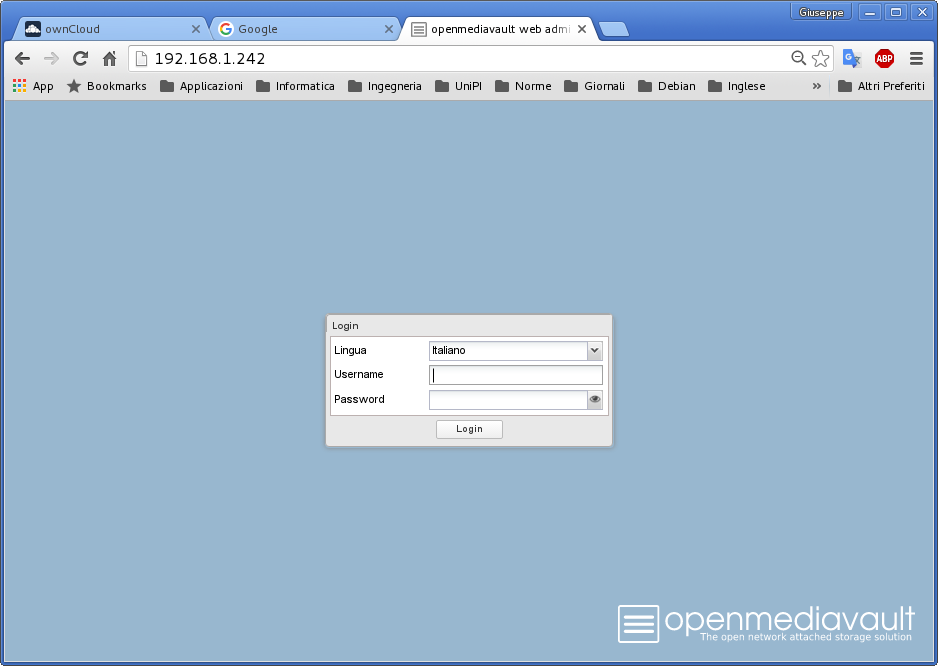
\includegraphics[width=0.7\textwidth]{OMV/OMVscreen.png}
\end{frame}

\begin{frame}
	\frametitle{Soluzioni OS: OpenMediaVault}
	\begin{columns}
		\begin{column}{0.48\textwidth}
			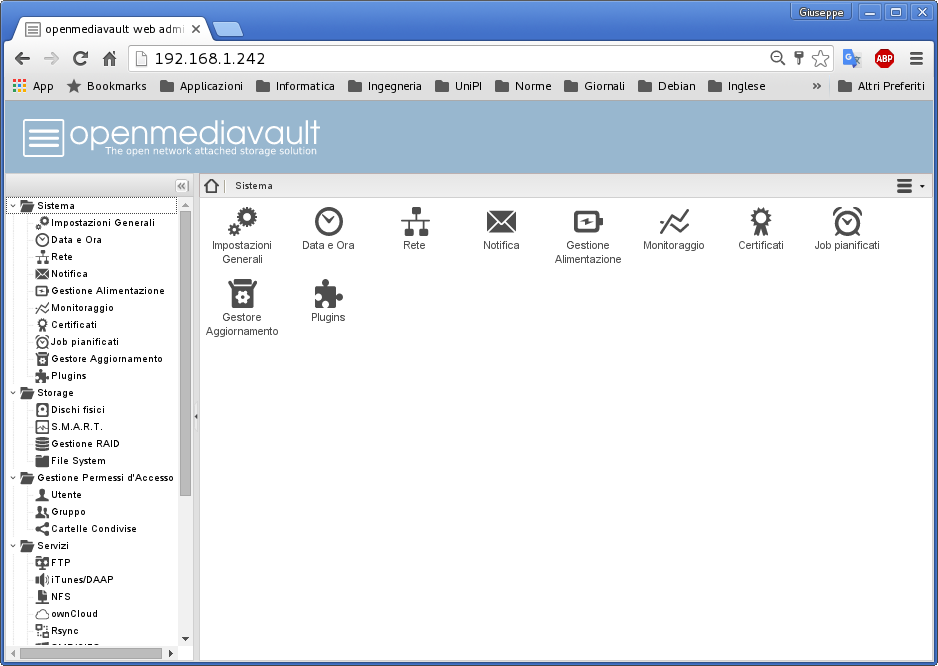
\includegraphics[width=\textwidth]{OMV/OMV1.png}
			\vspace{1mm}
			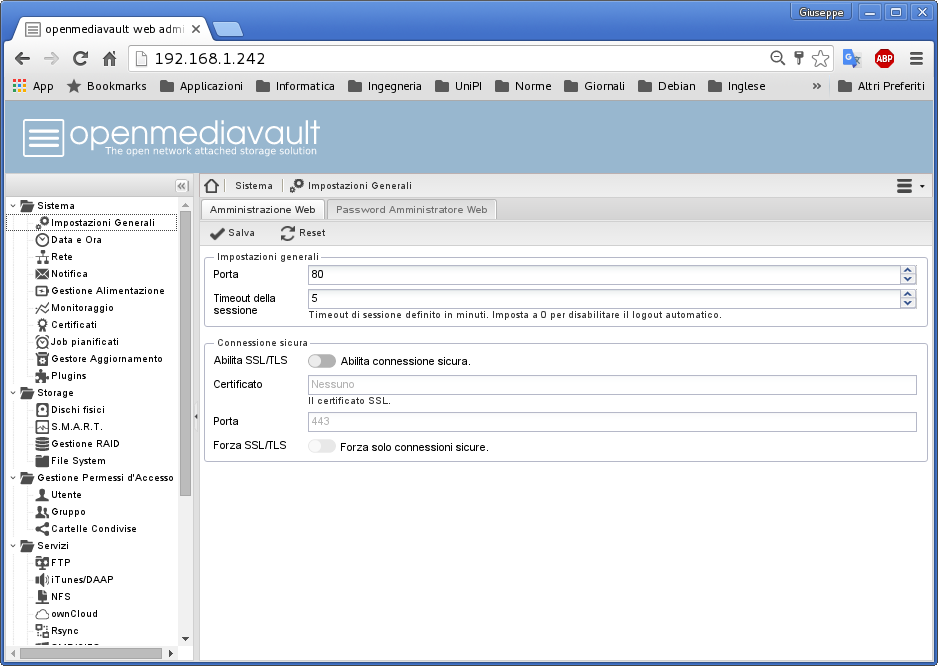
\includegraphics[width=\textwidth]{OMV/OMV3.png}
		\end{column}
		\begin{column}{0.48\textwidth}
			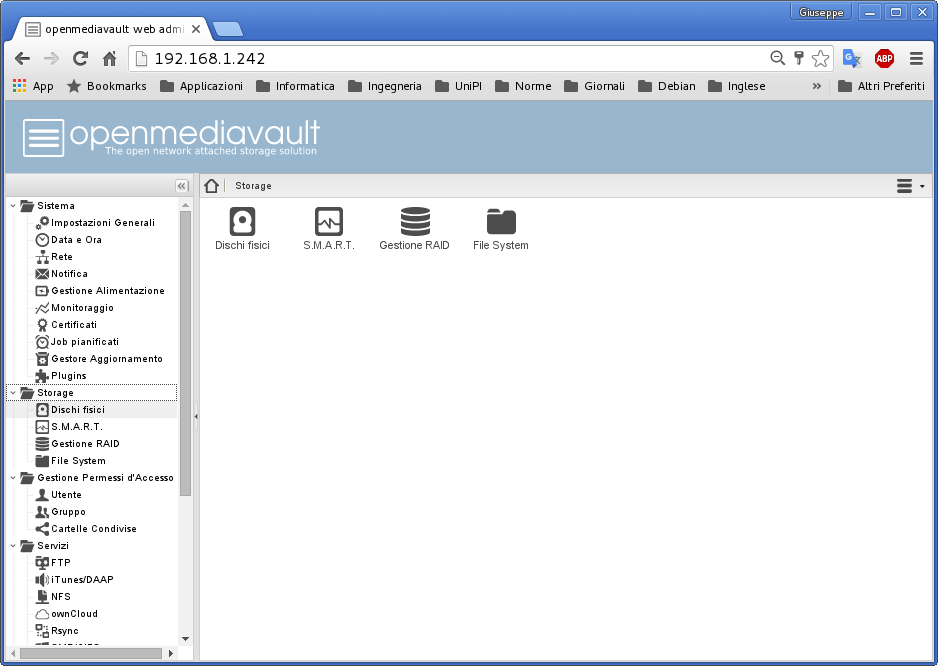
\includegraphics[width=\textwidth]{OMV/OMV4.png}
			\vspace{1mm}
			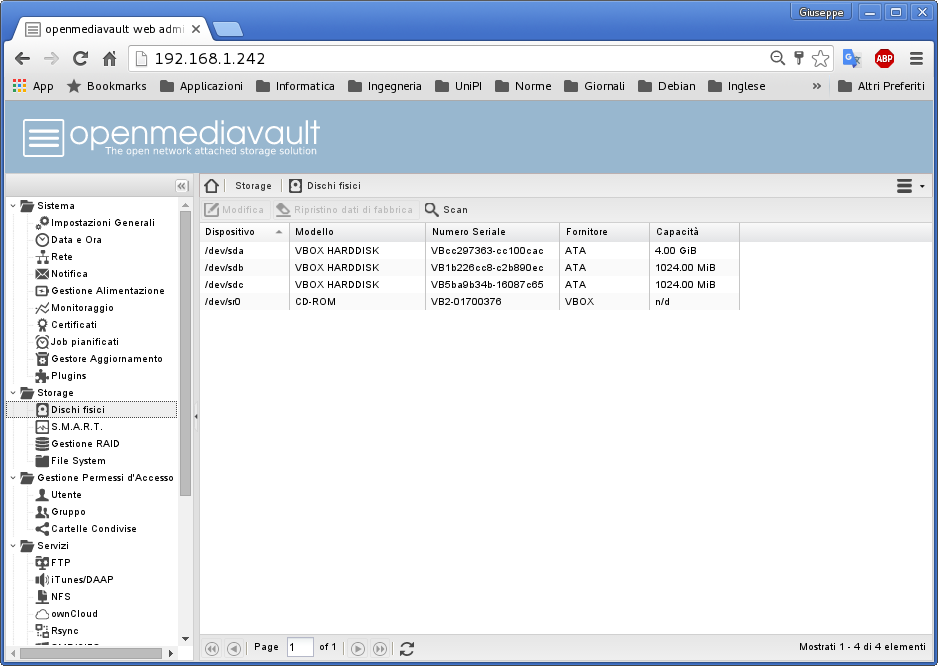
\includegraphics[width=\textwidth]{OMV/OMV5.png}
		\end{column}
	\end{columns}
\end{frame}

\begin{frame}
	\frametitle{Soluzioni OS: OpenMediaVault}
	\begin{columns}
		\begin{column}{0.48\textwidth}
			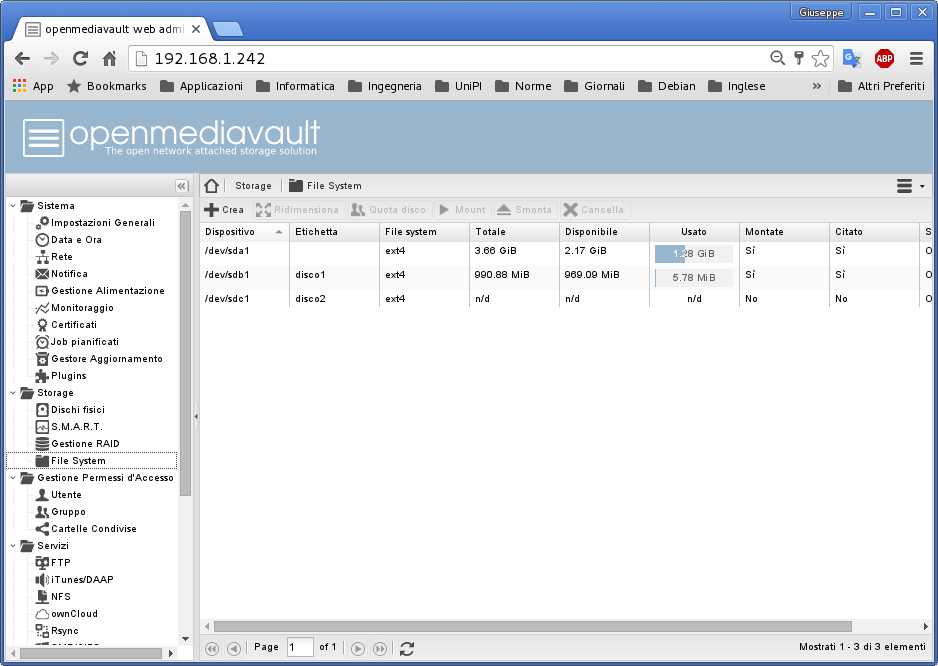
\includegraphics[width=\textwidth]{OMV/OMV6.png}
			\vspace{1mm}
			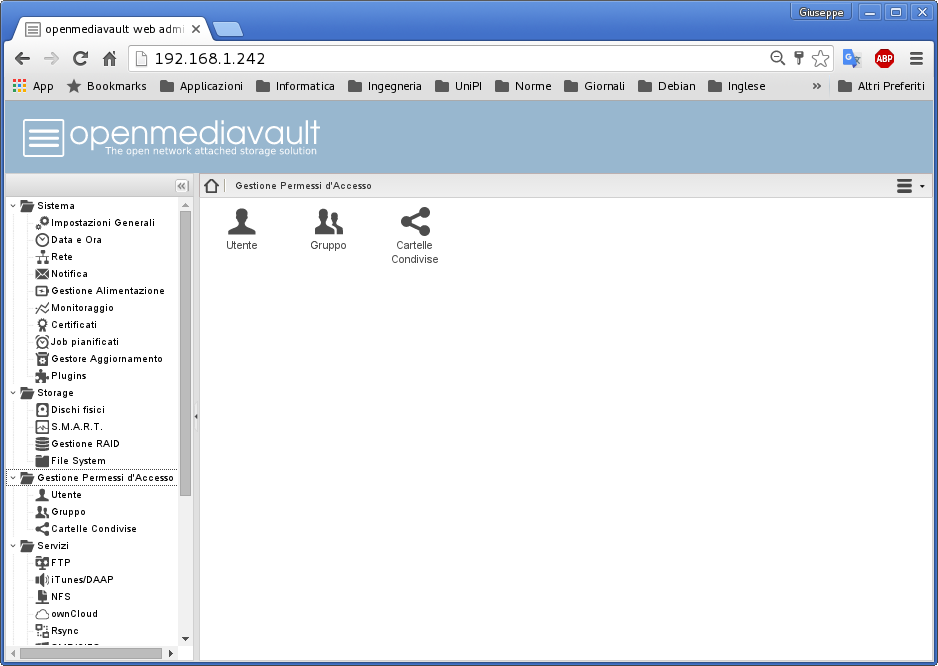
\includegraphics[width=\textwidth]{OMV/OMV7.png}
		\end{column}
		\begin{column}{0.48\textwidth}
			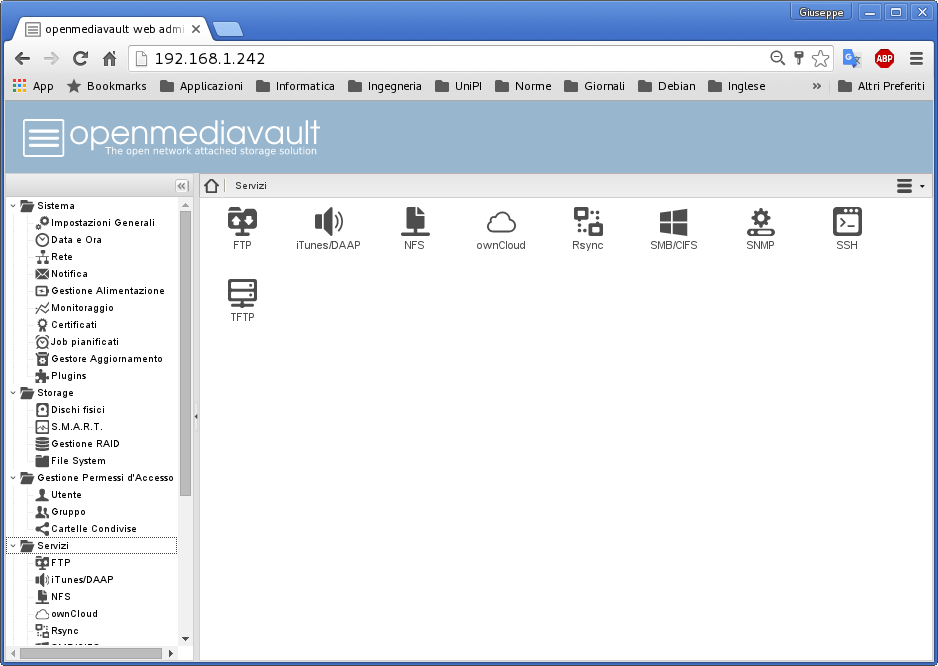
\includegraphics[width=\textwidth]{OMV/OMV8.png}
			\vspace{1mm}
			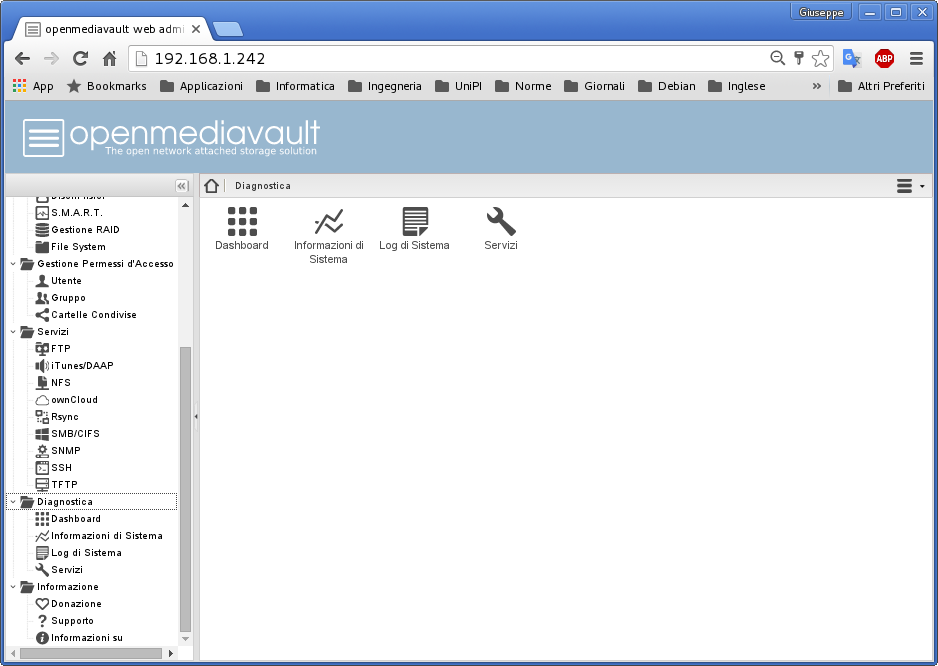
\includegraphics[width=\textwidth]{OMV/OMV9.png}
		\end{column}
	\end{columns}
\end{frame}

\subsection{OwnCloud}

\begin{frame}
	\frametitle{Una "nuvola" privata: OwnCloud}
	\begin{block}{da Wikipedia}
		\textbf{ownCloud} è un software libero che permette di gestire un completo servizio di file hosting.
	\end{block}
	\vspace{2mm}
	ownCloud rappresenta una alternativa al sistema Dropbox\textregistered che consente di avere funzioni analoghe con una memorizzazione locale delle informazioni. Permette di:
	\begin{itemize}
		\item mantenere il possesso dei propri files,
		\item organizzare il lavoro in modo distribuito all'interno della propria rete,
		\item distribuire contenuti multimediali (foto, musica, etc...) ed informazioni (calendari, bookmark, etc...)
	\end{itemize}

\end{frame}

\begin{frame}
	\frametitle{Una "nuvola" privata: OwnCloud}
	\begin{itemize}
		\item Sistema operativo base: quello che preferisco...
		\item accesso mediante WebGUI
		\item gestione a pacchetti dei plugins e delle applicazioni
	\end{itemize}
	\centering
	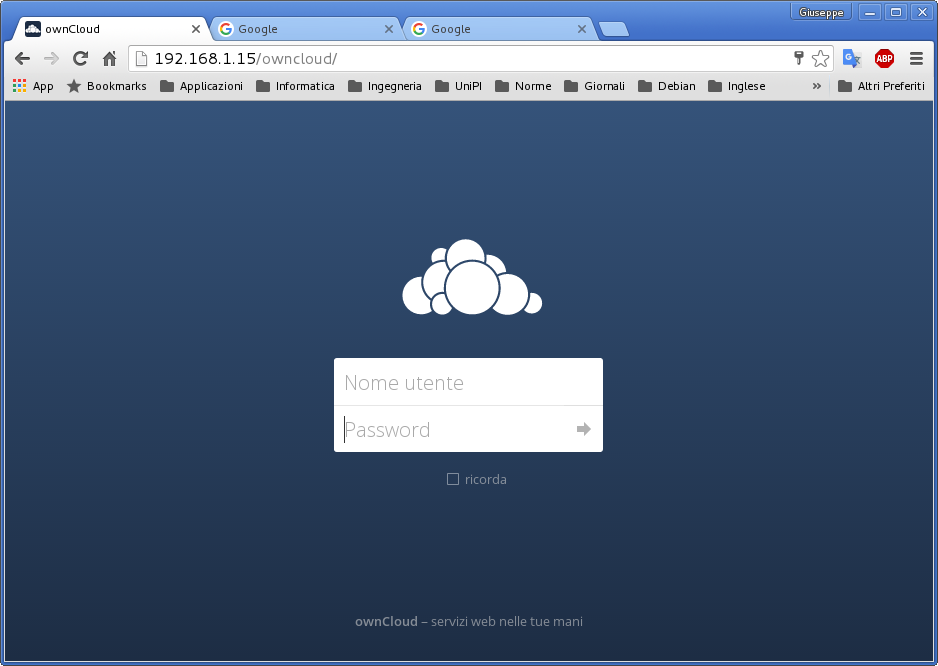
\includegraphics[width=0.7\textwidth]{OC/OC1.png}
\end{frame}

\begin{frame}
	\frametitle{Una "nuvola" privata: OwnCloud}
	\begin{columns}
		\begin{column}{0.48\textwidth}
			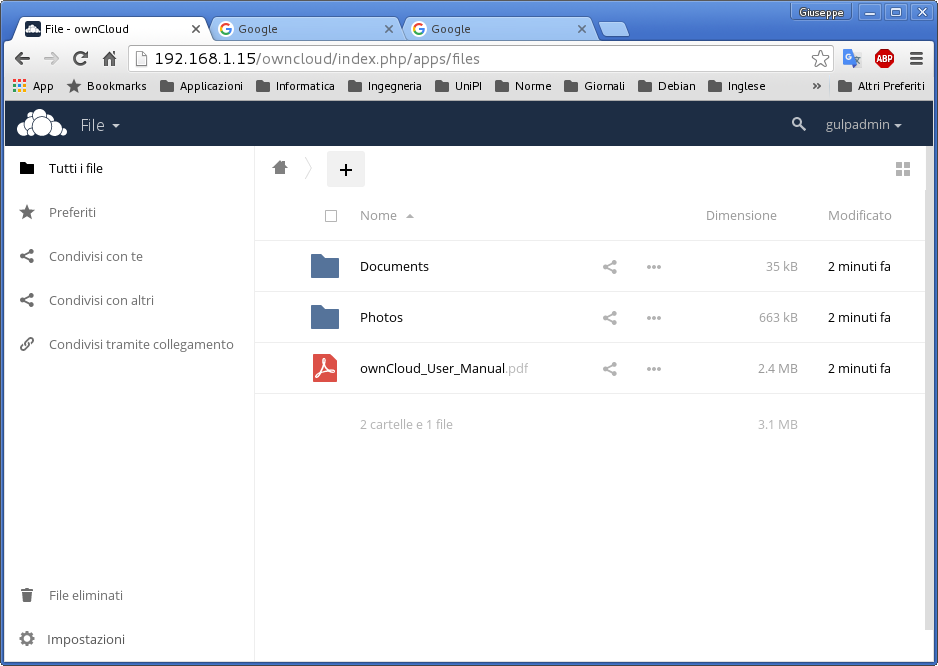
\includegraphics[width=\textwidth]{OC/OC2.png}
			\vspace{1mm}
			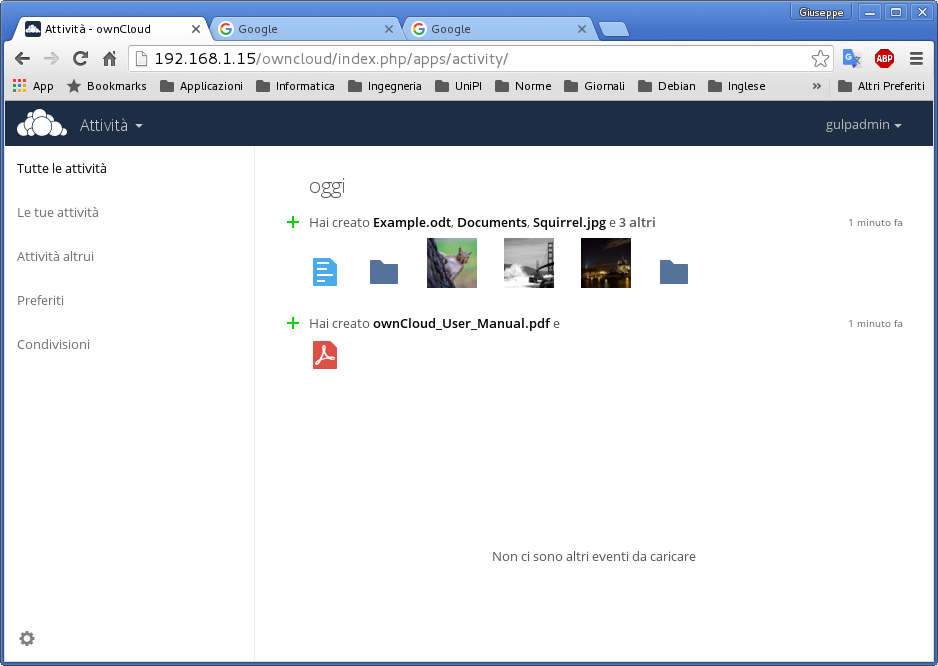
\includegraphics[width=\textwidth]{OC/OC3.png}
		\end{column}
		\begin{column}{0.48\textwidth}
			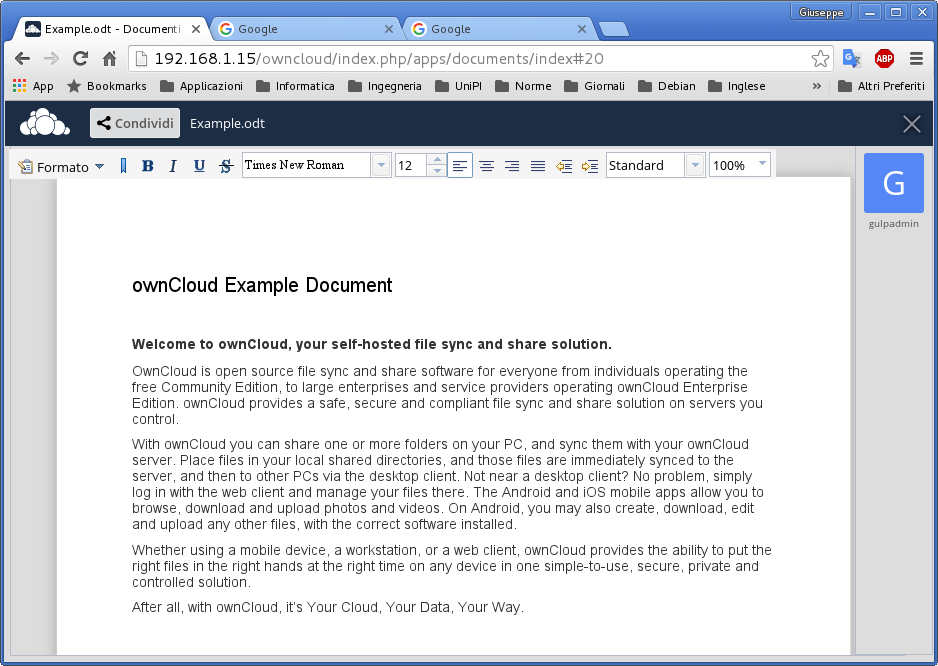
\includegraphics[width=\textwidth]{OC/OC4.png}
			\vspace{1mm}
			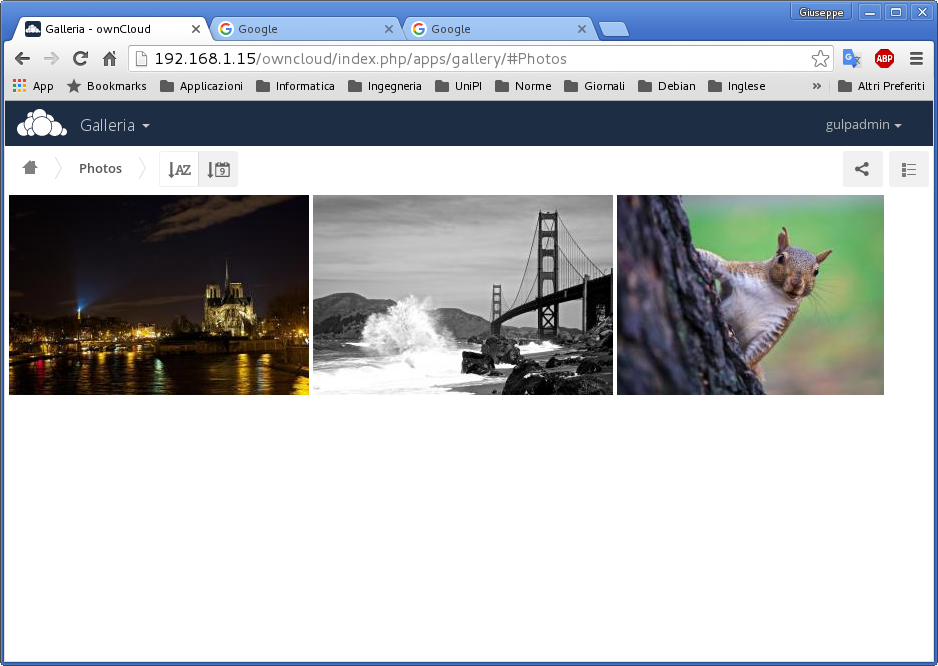
\includegraphics[width=\textwidth]{OC/OC5.png}
		\end{column}
	\end{columns}	
\end{frame}

\section{Note Conclusive}

\subsection{Materiale di consultazione}

\begin{frame}
	\frametitle{Materiale di consultazione}
	\begin{itemize}
		\item Web Site Nas4Free (\url{http://www.nas4free.org/})
		\item Nas4Free Wiki (\url{http://www.zoonsweb.nl/wiki/doku.php})
		\item Web Site FreeNAS (\url{http://www.freenas.org/})
		\item FreeNAS Documentation (\url{https://doc.freenas.org/})
		\item Web Site ownCloud (\url{https://owncloud.org/})
	\end{itemize}
\end{frame}

\subsection{Software usato per la presentazione}

\begin{frame}{Software per la presentazione}
	\frametitle{Software per la presentazione}
	\begin{block}{IMPORTANTE!!!}
		La presentazione è stata realizzata interamente mediante software LIBERO.
	\end{block}
	
	\begin{itemize}
		\item Latex con pacchetto Beamer\\ {\tiny (\url{https://www.ctan.org/tex-archive/macros/latex/contrib/beamer})}
		\item editor per LaTeX: TexStudio {\tiny (\url{http://www.texstudio.org/}) }
		\item Beamer Template: Laughlin by Mohamed El Morabity\\ {\tiny (\url{https://fedoraproject.org/wiki/Templates_for_Presentations})}
		\item Schema della rete: DIA {\tiny (\url{http://dia-installer.de/})}
		\item Elaborazione vettoriale delle figure: INKSCAPE\\ {\tiny (\url{https://inkscape.org/it/})}
		\item Virtualizzazione: Virtualbox {\tiny (\url{https://www.virtualbox.org/})}
	\end{itemize}
\end{frame}

\begin{frame}{Saluti}
	\frametitle{Saluti}
	\centering \textbf{\Large Domande?}\\
	\vspace{1cm}
	{Ci vediamo al prossimo seminario...}
	\begin{block}{24 febbraio 2016 – 21,30-22,30 – Saletta Ludoteca}
		Relatore: Massimo Pisani mydaq-large\\
		Titolo: Giochiamo con il National Instruments myDAQ
	\end{block}
\end{frame}


\end{document}
